%%%%%%%%%%%%%%%%%%%%%%%%%%%%%%%%%%%%%%%%%%%%%%%%%%%%%%%%%%%%%
%% Begin exercise %%
%%%%%%%%%%%%%%%%%%%%%%%%%%%%%%%%%%%%%%%%%%%%%%%%%%%%%%%%%%%%%
\ex{Transistor-based AC-DC converters}

%%%%%%%%%%%%%%%%%%%%%%%%%%%%%%%%%%%%%%%%%%%%%%%%%%%%%%%%%%%%%
%% Task 1: Single-phase inverter: %%
%%%%%%%%%%%%%%%%%%%%%%%%%%%%%%%%%%%%%%%%%%%%%%%%%%%%%%%%%%%%%

\task{Single-phase DC inverter}
The following ideal single-phase DC inverter
%%%%%%%%%%%%%%%%%%%%%%%%%%%%%%%%%%%%%%%%%%%%%%%%%%%%%%%%%%%%%
%% Single-phase DC inverter with inductive filter %%
%%%%%%%%%%%%%%%%%%%%%%%%%%%%%%%%%%%%%%%%%%%%%%%%%%%%%%%%%%%%%

\begin{figure}[htb]
    \begin{center}
        \begin{circuitikz}
            % Add voltage U1p
            \draw (0,0) coordinate (U1) to [open, o-o, v = $U_1\hspace{0.5cm}$, voltage = straight] ++(0,-5.5) coordinate (Gnd)
            % Add current
            (U1) to [short, o-, i=$i_1(t)$] ++(2,0) coordinate (jT1c)
            % Add T1
            (jT1c) to [Tnpn, n=T1, invert, bodydiode] ++(0,-2) coordinate (jT1e)
            % Add connection to u2
            (jT1e) to [short, *-] ++(1,0) to [crossing] ++(2,0) coordinate (ju2)
            % Add u2 inductor
            (ju2) to [L, l=$L$, name = L] ++(2,0)  to [short] ++(0.1,0) coordinate (ju2e)          
            % Add junction to T2
            (jT1e) to [short] ++(0,-1.5) coordinate (jT2c)
            % Add T2
            (jT2c) to [Tnpn, n=T2, invert, bodydiode] ++(0,-2) coordinate (jT2e)
            % Add connection to T3
            (jT1c) to [short, *-] ++(2,0) coordinate (jT3c)
            % Add T3
            (jT3c) to [Tnpn, n=T3, invert, bodydiode] ++(0,-2) coordinate (jT3e)
            % Add junction to ju2
            (jT3e) to [short] ++(0,-0.5) coordinate (jmu2)
            % Add junction to T4
            (jmu2) to [short] ++(0,-1) coordinate (jT4c)
            % Add T4
            (jT4c) to [Tnpn, n=T4, invert, bodydiode] ++(0,-2) coordinate (jT4e)
            % Add connection to T2
            (jT4e) to [short, -*] (jT2e)
            % Add connection to Gnd U1
            (jT2e) to [short, -] (Gnd)
            % Add connection to u2 inductor
            (jmu2) to [short,-] ++(0,2) coordinate (ju2x)
            % Add u2ae
            (ju2e) to [sV=$u_{2\mathrm{i}}(t)$] ++(0,-1.5) coordinate (ju2n)
            % Add connection of u2in
            (ju2n) to [short,-*] (jT4c);


            % Add component name of transistors
            \draw let \p1 = (T1.B) in node[anchor=east] at (\x1,\y1) {$T_1$};
            \draw let \p1 = (T2.B) in node[anchor=east] at (\x1,\y1) {$T_2$};
            \draw let \p1 = (T3.B) in node[anchor=east] at (\x1,\y1) {$T_3$};
            \draw let \p1 = (T4.B) in node[anchor=east] at (\x1,\y1) {$T_4$};
            % Add current arrows i2
            \draw (jT1e) ++(3,0) node[currarrow](i2){}
            (i2)  node[anchor=south,color=black]{$i_\mathrm{2}(t)$}
            % Add voltage arrows u2
            (ju2) ++(-0.5,0) to [open,v^=$$,voltage = straight] ++(0,-1.5)
            (ju2) ++ (0.1,-0.5) node[anchor=north,color=black]{$u_\mathrm{2}(t)$};
           % (ju2x) ++(0,-0.8) to [open,v^=$u_\mathrm{2}(t)$,voltage = straight] ++(3.8,0);
        \end{circuitikz}
    \end{center}
    \caption{Single-phase AC-DC converter}
    \label{fig:Fig_Single-phase_DC_Inverter}
\end{figure}

 

configured in a bridge topology and supplies a load consisting of an inductor and an internal load voltage. The inverter consists
of four thyristors arranged in H-bridge configuration.

\begin{table}[ht]
    \centering  % Zentriert die Tabelle
    \begin{tabular}{ll}
        \toprule
        Input DC voltage: & $U_{\mathrm{1}}=\SI{200}{\volt}$ \\
        Inductance: & $L = \SI{4.8}{\milli \henry}$ \\
        Internal load voltage: & $u_\mathrm{1e}(t) = 150 \sin(\omega t - \frac{\pi}{6})$ \\ 
        Reference angular frequency: & $\omega_2 = 2\pi \cdot \SI{50}{\hertz}$ \\ 
        \bottomrule
    \end{tabular}
    \caption{Parameters of the single-phase DC inverter.}  
    \label{table:ex07_Task1_ParametersOfTheCircuit}
\end{table}
The inverter is modulated using PWM with a modulation index of M=0.75.  Assuming ideal operation of the switching components:
% Subtask1
\subtask{Draw the inverter output voltage $u_\mathrm{2}(t)$ belonging to figure \ref{sfig:ex07_sub1.1_modulation}.
and its fundamental component $u^\mathrm{(1)}_\mathrm{2}(t)$. How large is the phase difference $\delta$ of the voltage
fundamental component $u^\mathrm{(1)}_\mathrm{2}(t)$ compared to the internal load voltage $u_\mathrm{1e}$?}

% Subtask2
\subtask{Calculate the amplitude $\hat{i}^\mathrm{(1)}_\mathrm{2}$ and the phase angle $\varphi^\mathrm{(1)}$ of the 
current fundamental wave $i^\mathrm{(1)}_\mathrm{2}(t)$ compared to $u_\mathrm{1e}$ and draw $u^\mathrm{(1)}_\mathrm{2}(t)$ 
and $i^\mathrm{(1)}_\mathrm{2}(t)$ in Fig. \ref{sfig:ex07_sub1.2_fund_components}.}

% Subtask3
\subtask{In Fig. \ref{sfig:ex07_sub1.3_Harmonics}, draw the voltage harmonics $u^\mathrm{(n)}_\mathrm{2}(t)$. Try to sketch, approximately,
the current harmonics $i^\mathrm{(n)}_\mathrm{2}(t)$ by counting the voltage time area squares. 
One square corresponds to a voltage time area of $\SI{17.8}{\milli \volt \second}$. The starting point is marked with \textbf{s}.\\

Hint:  The current harmonics $i^\mathrm{(n)}_\mathrm{2}(t)$ have no mean values.}

% Subtask4
\subtask{Draw the inverter's output current $i_\mathrm{2}(t)$, its fundamental wave $i^\mathrm{(1)}_\mathrm{2}(t)$ 
and its harmonics $i^\mathrm{(n)}_\mathrm{2}(t)$ in Fig. \ref{sfig:ex07_sub1.4_current_and_components}.}

% Subtask5
\subtask{Mark the input current $i_\mathrm{i}(t)$ of the DC voltage inverter in the same figure of subtask 2.1.4.}
%\begin{figure}[htb]
%    \begin{center}
%        \begin{circuitikz}
%            \begin{scope}[yshift=-9cm, local bounding box=sawtooth]
                %\draw (0,-1) -- ++(0,2) -- ++(2,-2) -- ++(0,2) -- ++(2,-2) -- ++(0,2) -- ++(2,-2);
                % the above line does the same as the following one, but without the foreach loop
%                \draw (0,-1) foreach \x in {1,2,3} {-- ++(2,2) -- ++(0,-2) };
%            \end{scope}
%        \end{circuitikz}
%    \end{center}
%    \caption{Single-phase DC Inverter}
   % \label{fig:Fig_Single-phase_DC_Inverter}
%\end{figure}
%%%%%%%%%%%%%%%%%%%%%%%%%%%%%%%%%%%%%%%%%%%%%%%%%%%%%%%%%%%%%%%%%%%%%%%%%%
% Fundamental Current i^1_1a for M3C with RL-Load
%%%%%%%%%%%%%%%%%%%%%%%%%%%%%%%%%%%%%%%%%%%%%%%%%%%%%%%%%%%%%%%%%%%%%%%%%%
\begin{figure}[htb]

    %   \documentclass{standalone}
    %   \usepackage{pgfplots}
    %   \pgfplotsset{compat=1.18} % Kompatibilität für neuere Versionen
           \centering
           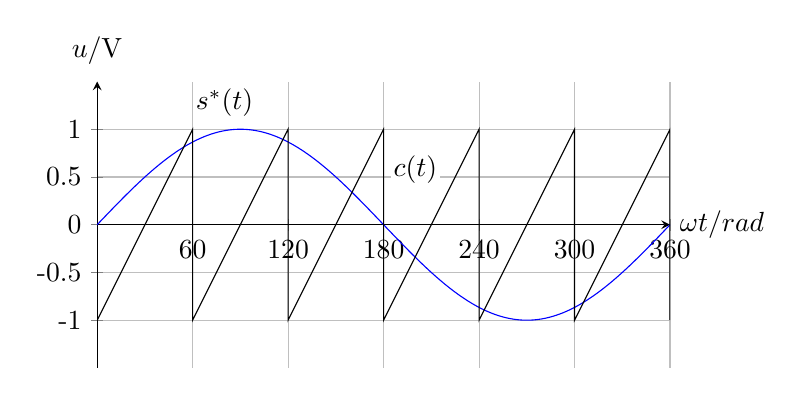
\begin{tikzpicture}
                \pgfplotsset{set layers}
           \begin{axis}[
            % x/y range adjustment
            scale only axis,
            ymin=-1.5, ymax=1.5,
            xmin=0, xmax=360, 
            samples=500,
            axis y line=center,
            axis x line=middle,
            extra y ticks=0,
            % Label text
            xlabel={$\omega t / \text{rad}$},
            ylabel={$u/\mathrm{V}$},
            % Label adjustment
            x label style={at={(axis description cs:1,0.5)},anchor=west},
            y label style={at={(axis description cs:0,.97)},anchor=south,yshift=0.2cm},
            width=0.6\textwidth,
            height=0.3\textwidth,
            % x-Ticks
            xtick={0,60,120,180,240, 300, 360},
            xticklabels={0,60,120,180,240, 300, 360},
            xticklabel style = {anchor=north},
            % y-Ticks
            ytick={-1,-0.5,0,0.5,1},
            yticklabels={-1,-0.5,0,0.5,1},
            yticklabel style = {anchor=east},
            % Grid layout
            grid,
            %grid style={line width=.1pt, draw=gray!10},
            %major grid style={line width=.2pt,draw=gray!90},
        ] 
        % modulation s
        \addplot[blue, domain= 0:360, solid] {sin(x)};
      % carrier signal c
       \draw[thin, black] (0,-1) -- (60,1) -- (60,-1) -- (120,1) -- (120,-1) -- (180,1) -- (180,-1) -- (240,1) -- (240,-1) -- (300,1) -- (300,-1) -- (360,1) -- (360,-1);
        %\draw (0,-1) \foreach \x in {0 ,60, 120, 180, 240, 300} {-- ++(60,2) -- ++(0,-2) };
        
        % Label of s
        \node[black, fill=white, inner sep = 1pt, anchor = south] at (axis cs:80,1.1) {$s^{*}(t)$};
        % Label of c
        \node[black, fill=white, inner sep = 1pt, anchor = south] at (axis cs:200,0.4) {$c(t)$};
           \end{axis}         
           \end{tikzpicture}
           \caption{Carrier signal $c(t)$ and reference $s^{*}(t)$.}
           \label{sfig:ex07_sub1.1_modulation}
   \end{figure} 
%%%%%%%%%%%%%%%%%%%%%%%%%%%%%%%%%%%%%%%%%%%%%%%%%%%%%%%%%%%%%%%%%%%%%%%%%%%%%%%%%%%%%
% Fundamental Current i^1_1 and fundamental volage u^1_2 for single-phase DC inverter
%%%%%%%%%%%%%%%%%%%%%%%%%%%%%%%%%%%%%%%%%%%%%%%%%%%%%%%%%%%%%%%%%%%%%%%%%%%%%%%%%%%%%
\begin{figure}[h!]

    %   \documentclass{standalone}
    %   \usepackage{pgfplots}
    %   \pgfplotsset{compat=1.18} % Kompatibilität für neuere Versionen
           \centering
           \begin{tikzpicture}
                \pgfplotsset{set layers}
           \begin{axis}[
            % x/y range adjustment
            scale only axis,
            ymin=-200, ymax=200,
            xmin=0, xmax=360, 
            samples=500,
            axis y line=center,
            axis x line=middle,
            extra y ticks=0,
            % Label text
            xlabel={$\omega t / \text{rad}$},
            ylabel={$u/\mathrm{V}$},
            % Label adjustment
            x label style={at={(axis description cs:1.05,0.5)},anchor=west},
            y label style={at={(axis description cs:0,.97)},anchor=south,yshift=0.2cm},
            width=0.6\textwidth,
            height=0.3\textwidth,
            % x-Ticks
            xtick={0,60,120,180,240, 300, 360},
            xticklabels={0,$\frac{\pi}{3}$,$\frac{2\pi}{3}$,$\pi$,$\frac{4\pi}{3}$, $\frac{5\pi}{3}$, $2\pi$},
            xticklabel style = {anchor=north},
            % y-Ticks
            ytick={-200,-100,0,100,200},
            yticklabels={-200,-100,0,100,200},
            yticklabel style = {anchor=east},
            % Grid layout
            grid,
            thick
            %grid style={line width=.1pt, draw=gray!10},
            %major grid style={line width=.2pt,draw=gray!90},
        ] 
        % internal load voltage u_2i
        \addplot[signalalpha, domain= 0:360, solid, thick] {150*sin(x-(180/6))};
        % Label of u_2i
        \node[signalalpha, fill=white, inner sep = 1pt, anchor = south] at (axis cs:120,160) {$u_{2\mathrm{i}}(t)$};
        \begin{solutionblock}
        % fundamental voltage u^(1)_2
        \addplot[signalbeta, domain= 0:360, solid, thick] {150*sin(x)};
         % Label of u^(1)_2
         \node[signalbeta, fill=white, inner sep = 1pt, anchor = south] at (axis cs:70,155) {$u^\mathrm{(1)}_\mathrm{2}(t)$};
        \end{solutionblock}
           \end{axis}
           \begin{axis}[
            % x/y range adjustment
            scale only axis,
            ymin=-100, ymax=100,
            xmin=0, xmax=360,
            axis x line=none, 
            samples=500,
            axis y line=right,
            axis x line=middle,
            extra y ticks=0,
            % Label text
            ylabel={$i/\mathrm{A}$},
            % Label adjustment
            y label style={rotate = -90,at={(axis description cs:1,.97)},anchor=south,yshift=0.2cm},
            width=0.6\textwidth,
            height=0.3\textwidth,
            % y-Ticks
            ytick={-100,-50,0,50,100},
            yticklabels={-100,-50,0,50,100},
            yticklabel style = {anchor=west},
            % Grid layout
            grid,
            thick
            %grid style={line width=.1pt, draw=gray!10},
            %major grid style={line width=.2pt,draw=gray!90},
        ]
        \begin{solutionblock}
              % fundamental current i^(1)_2
              \addplot[signaldelta, domain= 0:360, solid, thick] {51.5*sin(x-14.9)};
                % Label of i^(1)_2
                \node[signaldelta, fill=white, inner sep = 1pt, anchor = south] at (axis cs:100,25) {$i^\mathrm{(1)}_\mathrm{2}(t)$};
            \end{solutionblock}
           \end{axis}             
           \end{tikzpicture}
           \caption{Internal load voltage $u_{2\mathrm{i}}(t)$, fundamental voltage and current components $u^\mathrm{(1)}_\mathrm{2}(t)$
            and  $i^\mathrm{(1)}_\mathrm{2}(t)$, respectively. }
           \label{sfig:ex07_sub1.2_fund_components}
   \end{figure}
%%%%%%%%%%%%%%%%%%%%%%%%%%%%%%%%%%%%%%%%%%%%%%%%%%%%%%%%%%%%%%%%%%%%%%%%%%%%%%%%%%%%%
% Fundamental Current i^1_1 and fundamental volage u^1_2 for single-phase DC inverter
%%%%%%%%%%%%%%%%%%%%%%%%%%%%%%%%%%%%%%%%%%%%%%%%%%%%%%%%%%%%%%%%%%%%%%%%%%%%%%%%%%%%%
\begin{figure}[h!]

    %   \documentclass{standalone}
    %   \usepackage{pgfplots}
    %   \pgfplotsset{compat=1.18} % Kompatibilität für neuere Versionen
           \centering
           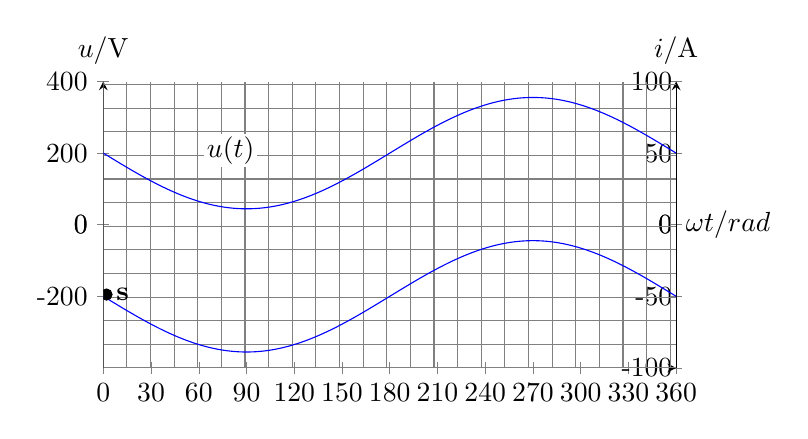
\begin{tikzpicture}
                \pgfplotsset{set layers}
           \begin{axis}[
            % x/y range adjustment
            scale only axis,
            ymin=-400, ymax=400,
            xmin=0, xmax=540, 
            samples=500,
            axis y line=center,
            axis x line=bottom,
            extra y ticks=0,
            % Label text
            xlabel={$\omega t / \text{rad}$},
            ylabel={$u/\mathrm{V}$},
            % Label adjustment
            x label style={at={(axis description cs:1,0.5)},anchor=west},
            y label style={at={(axis description cs:0,.97)},anchor=south,yshift=0.2cm},
            width=0.6\textwidth,
            height=0.3\textwidth,
            % x-Ticks
            xtick={0, 45, 90, 135, 180, 225, 270, 315, 360, 405, 450,495, 540},
            xticklabels={0, 30, 60, 90, 120, 150, 180, 210, 240, 270, 300, 330, 360},
            xticklabel style = {anchor=north},
            % y-Ticks
            ytick={-400,-200,0,200,400},
            yticklabels={-400,-200,0,200,400},
            yticklabel style = {anchor=east},
            % Grid layout
           % grid,
            %grid style={line width=.1pt, draw=gray!10},
            %major grid style={line width=.2pt,draw=gray!90},
        ] 
        % Grid
        \draw[step=0.3cm, gray, thin] (0,-400) grid (540,400);
        % internal load voltage u
        \addplot[blue, domain= 0:540, solid] {-155.5*sin(x/1.5)+200};
        \addplot[blue, domain= 0:540, solid] {-155.5*sin(x/1.5)-200};
         % Label of u
         \node[black, fill=white, inner sep = 1pt, anchor = south] at (axis cs:120,160) {$u(t)$};
         % Start point
         \filldraw[black] (3,-195) circle (2pt) node[anchor=west]{\textbf{s}};
           \end{axis}
           \begin{axis}[
            % x/y range adjustment
            scale only axis,
            ymin=-100, ymax=100,
            xmin=0, xmax=360,
            axis x line=none, 
            samples=500,
            axis y line=right,
            axis x line=middle,
            extra y ticks=0,
            % Label text
            ylabel={$i/\mathrm{A}$},
            % Label adjustment
            y label style={rotate = -90,at={(axis description cs:1,.97)},anchor=south,yshift=0.2cm},
            width=0.6\textwidth,
            height=0.3\textwidth,
            % y-Ticks
            ytick={-100,-50,0,50,100},
            yticklabels={-100,-50,0,50,100},
            yticklabel style = {anchor=east},
            % Grid layout
           % grid,
            %grid style={line width=.1pt, draw=gray!10},
            %major grid style={line width=.2pt,draw=gray!90},
        ]
           \end{axis}             
           \end{tikzpicture}
           \caption{Harmonics of the output voltage and current.}
           \label{sfig:ex07_sub1.3_Harmonics}
   \end{figure}
%%%%%%%%%%%%%%%%%%%%%%%%%%%%%%%%%%%%%%%%%%%%%%%%%%%%%%%%%%%%%%%%%%%%%%%%%%%%%%%%%%%%%
% Fundamental Current i^1_1 and fundamental volage u^1_2 for single-phase DC inverter
%%%%%%%%%%%%%%%%%%%%%%%%%%%%%%%%%%%%%%%%%%%%%%%%%%%%%%%%%%%%%%%%%%%%%%%%%%%%%%%%%%%%%
\begin{figure}[h]

    %   \documentclass{standalone}
    %   \usepackage{pgfplots}
    %   \pgfplotsset{compat=1.18} % Kompatibilität für neuere Versionen
           \centering
           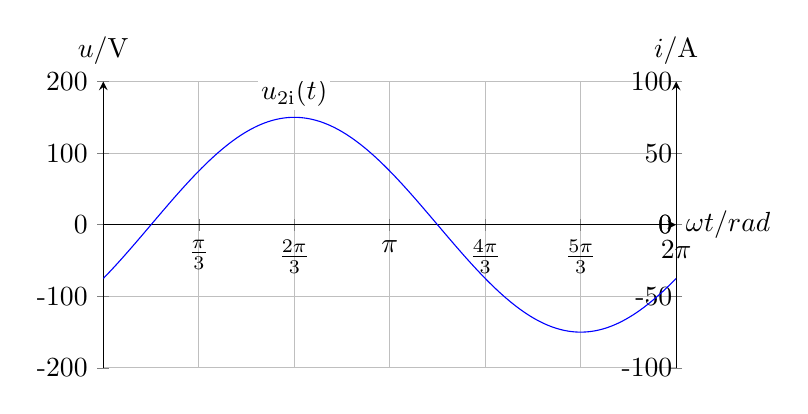
\begin{tikzpicture}
                \pgfplotsset{set layers}
           \begin{axis}[
            % x/y range adjustment
            scale only axis,
            ymin=-200, ymax=200,
            xmin=0, xmax=360, 
            samples=500,
            axis y line=center,
            axis x line=middle,
            extra y ticks=0,
            % Label text
            xlabel={$\omega t / \text{rad}$},
            ylabel={$u/\mathrm{V}$},
            % Label adjustment
            x label style={at={(axis description cs:1,0.5)},anchor=west},
            y label style={at={(axis description cs:0,.97)},anchor=south,yshift=0.2cm},
            width=0.6\textwidth,
            height=0.3\textwidth,
            % x-Ticks
            xtick={0,60,120,180,240, 300, 360},
            xticklabels={0,$\frac{\pi}{3}$,$\frac{2\pi}{3}$,$\pi$,$\frac{4\pi}{3}$, $\frac{5\pi}{3}$, $2\pi$},
            xticklabel style = {anchor=north},
            % y-Ticks
            ytick={-200,-100,0,100,200},
            yticklabels={-200,-100,0,100,200},
            yticklabel style = {anchor=east},
            % Grid layout
            grid,
            %grid style={line width=.1pt, draw=gray!10},
            %major grid style={line width=.2pt,draw=gray!90},
        ] 
        % internal load voltage u
        \addplot[blue, domain= 0:360, solid] {150*sin(x-(180/6))};
         % Label of u
         \node[black, fill=white, inner sep = 1pt, anchor = south] at (axis cs:120,160) {$u_{2\mathrm{i}}(t)$};
           \end{axis}
           \begin{axis}[
            % x/y range adjustment
            scale only axis,
            ymin=-100, ymax=100,
            xmin=0, xmax=360,
            axis x line=none, 
            samples=500,
            axis y line=right,
            axis x line=middle,
            extra y ticks=0,
            % Label text
            ylabel={$i/\mathrm{A}$},
            % Label adjustment
            y label style={rotate = -90,at={(axis description cs:1,.97)},anchor=south,yshift=0.2cm},
            width=0.6\textwidth,
            height=0.3\textwidth,
            % y-Ticks
            ytick={-100,-50,0,50,100},
            yticklabels={-100,-50,0,50,100},
            yticklabel style = {anchor=east},
            % Grid layout
            grid,
            %grid style={line width=.1pt, draw=gray!10},
            %major grid style={line width=.2pt,draw=gray!90},
        ]
           \end{axis}             
           \end{tikzpicture}
           \caption{Output current $i_\mathrm{2}(t)$, its fundamental wave $i^\mathrm{(1)}_\mathrm{2}(t)$ 
           and its harmonics $i^{(k)}_\mathrm{2}(t)$. }
           \label{sfig:ex07_sub1.4_current_and_components}
   \end{figure}
\newpage

%%%%%%%%%%%%%%%%%%%%%%%%%%%%%%%%%%%%%%%%%%%%%%%%%%%%%%%%%%%%%
%% Task 2: Three-phase inverter in six-step mode         %%
%%%%%%%%%%%%%%%%%%%%%%%%%%%%%%%%%%%%%%%%%%%%%%%%%%%%%%%%%%%%%

\task{Symmetrical 3-phase switching rectifier}

An symmetrical switching rectifier in three-phase bridge topology shall supply a
symmetrical three-phase consumer. The consumer is simulated by an inductance and 
a sinusoidal counter voltage per phase. The inverter is operated with a basic frequency clock.
The switching elements are considered as ideal.

% %%%%%%%%%%%%%%%%%%%%%%%%%%%%%%%%%%%%%%%%%%%%%%%%%%%%%%%%%%%%%%%%%%%%%%%
 % Fig_ThreePhaseInverter_6StepMode
%%%%%%%%%%%%%%%%%%%%%%%%%%%%%%%%%%%%%%%%%%%%%%%%%%%%%%%%%%%%%%%%%%%%%%%
    \begin{figure}[htb]
        \begin{center}
            \begin{circuitikz}
                % Add voltage U1p
                \draw (0,0) coordinate (U1p) to [open, o-o, v = $\frac{U_1}{2}\hspace{0.5cm}$, voltage = straight] ++(0,-2.5) coordinate (Gnd)
                (Gnd) node[rground, rotate = 270 ](){} ++(0.4,0)
                (Gnd) to [open, -o, v = $\frac{U_1}{2}\hspace{0.5cm}$, voltage = straight] ++(0,-2.5) coordinate (U1m)
                % Add current
                (U1p) to [short, o-, i=$i_1(t)$] ++(2,0) coordinate (jT1c)
                % Add T1
                (jT1c) to [Tnpn, n=T1, invert, bodydiode] ++(0,-2) coordinate (jT1e)
                % Add connection to u2a
                (jT1e) to [short, *-] ++(1,0) to [crossing] ++(2,0) to [crossing] ++(2,0) to [short,-] ++(3,0) coordinate (ju2a)          
                % Add junction to T2
                (jT1e) to [short] ++(0,-1) coordinate (jT2c)
                % Add T2
                (jT2c) to [Tnpn, n=T2, invert, bodydiode] ++(0,-2) coordinate (jT2e)
                % Add connection to T3
                (jT1c) to [short, *-] ++(2,0) coordinate (jT3c)
                % Add T3
                (jT3c) to [Tnpn, n=T3, invert, bodydiode] ++(0,-2) coordinate (jT3e)
                % Add junction to ju2b
                (jT3e) to [short] ++(0,-0.5) coordinate (jmu2b)
                % Add connection to u1b
                (jmu2b) to [short,*-] ++(1,0) to [crossing] ++(2,0) to [short,-] ++(3,0) coordinate (ju2b)
                % Add junction to T4
                (jmu2b) to [short] ++(0,-0.5) coordinate (jT4c)
                % Add T4
                (jT4c) to [Tnpn, n=T4, invert, bodydiode] ++(0,-2) coordinate (jT4e)
                % Add connection to T5
                (jT3c) to [short, *-] ++(2,0) coordinate (jT5c)
                % Add T5
                (jT5c) to [Tnpn, n=T5, invert, bodydiode] ++(0,-2) coordinate (jT5e)
                % Add junction to T6
                (jT5e) to [short] ++(0,-1) coordinate (jT6c)
                % Add T6
                (jT6c) to [Tnpn, n=T6, invert, bodydiode] ++(0,-2) coordinate (jT6e)
                % Add connection to T4
                (jT6e) to [short, -*] (jT4e)
                % Add connection to T2
                (jT4e) to [short, -*] (jT2e)
                % Add connection to U1m
                (jT2e) to [short, -] (U1m)
                % Add 2. Ground symbol
                (jmu2b) ++(4.7,-2.6) node[rground](){} coordinate (Gnd2)
                % Add connection to u2c
                (jT6c) to [short,*-] ++(4,0) coordinate (ju2c)
                % Add connection to u2a inductor
                (ju2a) to [short,-] ++(0,2) coordinate (ju2ax)
                % Add u2a inductor
                (ju2ax) to [L, l=$L$, name = L] ++(2,0) coordinate (ju2ae)
                % Add u2ae
                 (ju2ae) to [sV=$u_\mathrm{2ai}$] ++(1.5,0) coordinate (ju2an)
                % Add u2b inductor
                (ju2b) to [L, l=$L$, name = L] ++(2,0) coordinate (ju2be)
                % Add u2be
                 (ju2be) to [sV=$u_\mathrm{2bi}$] ++(1.5,0) coordinate (ju2bn)
                % Add connection to u2c inductor
                (ju2c) to [short,-] ++(0,-2) coordinate (ju2cx)
                % Add u2a inductor
                (ju2cx) to [L, l=$L$, name = L] ++(2,0) coordinate (ju2ce)
                % Add u2ce
                (ju2ce) to [sV=$u_\mathrm{2ci}$] ++(1.5,0) coordinate (ju2cn)
                % Add connection of u2in
                (ju2an) to [short,-*] (ju2bn) to [short,-] (ju2cn)
                % Add connection point u2n
                (ju2bn) to [short,-o] ++(0.6,0) coordinate (ju2n)
                % Add 3. Ground symbol
                (ju2n) ++(0,-2.6) node[rground](){} coordinate (Gnd3);


                % Add component name of transistors
                \draw let \p1 = (T1.B) in node[anchor=east] at (\x1,\y1) {$T_1$};
                \draw let \p1 = (T2.B) in node[anchor=east] at (\x1,\y1) {$T_2$};
                \draw let \p1 = (T3.B) in node[anchor=east] at (\x1,\y1) {$T_3$};
                \draw let \p1 = (T4.B) in node[anchor=east] at (\x1,\y1) {$T_4$};
                \draw let \p1 = (T5.B) in node[anchor=east] at (\x1,\y1) {$T_5$};
                \draw let \p1 = (T6.B) in node[anchor=east] at (\x1,\y1) {$T_6$};
                % Add current arrows i2a, i2b and i2c
                \draw (jT1e) ++(1,0) node[currarrow](i2a){}
                (i2a)  node[anchor=north,color=black]{$i_\mathrm{2a}(t)$}
                (jmu2b) ++(1,0) node[currarrow](i2b){}
                (i2b)  node[anchor=north,color=black]{$i_\mathrm{2b}(t)$}
                (jT6c) ++(1,0) node[currarrow](i2c){}
                (i2c)  node[anchor=north,color=black]{$i_\mathrm{2c}(t)$}
                % Add voltage arrow u1
                (U1p) ++(0.3,0.5) to [open,v^=$$,voltage = straight] ++(0,-6)coordinate (Uges)
                (Uges) ++ (0.3,3) node[anchor=north,color=black]{$U_\mathrm{1}$}
                % Add voltage arrow u2an, u2bn and u2cn
                (ju2ax) ++(0,-0.8) to [open,v^=$u_\mathrm{2a}(t)$, voltage = straight] ++(3.8,0)
                (ju2b) ++(0,-0.8) to [open,v^=$u_\mathrm{2b}(t)$,voltage = straight] ++(3.8,0)
                (ju2cx) ++(0,-0.8) to [open,v^=$u_\mathrm{2c}(t)$,voltage = straight] ++(3.8,0)
                % Add voltage arrow u2ab
                (ju2ax) ++(0.2,0) to [open,v^=$$,voltage = straight] ++(0,-2.5)
                (ju2ax) ++ (0.9,-1) node[anchor=north,color=black]{$u_\mathrm{2ab}(t)$}
                % Add voltage arrow u2bc
                (ju2b) ++(0.2,0) to [open,v^=$$,voltage = straight] ++(0,-2.5)
                (ju2b) ++ (0.9,-1) node[anchor=north,color=black]{$u_\mathrm{2bc}(t)$}
                % Add voltage arrow ua0
                (Gnd2) ++(-0.7,3.4) to [open,v^=$$,voltage = straight] ++(0,-3.6)
                (Gnd2) ++ (-1.4,1.2) node[anchor=north,color=black,rotate = 90]{$u_\mathrm{2a0}(t)$}
                % Add voltage arrow ub0
                (Gnd2) ++(0,2.9) to [open,v^=$$,voltage = straight] ++(0,-3.01)
                (Gnd2) ++ (-0.7,1.2) node[anchor=north,color=black,rotate = 90]{$u_\mathrm{2b0}(t)$}
                % Add voltage arrow uc0
                (Gnd2) ++(0.7,2.4) to [open,v^=$$,voltage = straight] ++(0,-2.42)
                (Gnd2) ++ (0,1.2) node[anchor=north,color=black,rotate = 90]{$u_\mathrm{2b0}(t)$}
                % Add voltage arrow un0
                (Gnd3) ++(0,2.8) to [open,v^=$$,voltage = straight] ++(0,-3.01)
                (Gnd3) ++ (-0.7,1.2) node[anchor=north,color=black,rotate = 90]{$u_\mathrm{2n0}(t)$};



            \end{circuitikz}
        \end{center}
        \caption{Three-phase inverter in six-step mode.}
        \label{fig:Fig_ThreePhaseInverter_6StepMode}
    \end{figure}



%%%%%%%%%%%%%%%%%%%%%%%%%%%%%%%%%%%%%%%%%%%%%%%%%%%%%%%%%%%%%%%%%%%%%%%
 % Fig_ThreePhaseInverter_6StepMode
%%%%%%%%%%%%%%%%%%%%%%%%%%%%%%%%%%%%%%%%%%%%%%%%%%%%%%%%%%%%%%%%%%%%%%%
    \begin{figure}[htb]
        \begin{center}
            \begin{circuitikz}
                % Add voltage U1p
                \draw (0,0) coordinate (U1p) to [open, o-o, v = $\frac{U_1}{2}\hspace{0.5cm}$, voltage = straight] ++(0,-2.5) coordinate (Gnd)
                (Gnd) node[rground, rotate = 270 ](){} ++(0.4,0)
                (Gnd) to [open, -o, v = $\frac{U_1}{2}\hspace{0.5cm}$, voltage = straight] ++(0,-2.5) coordinate (U1m)
                % Add current
                (U1p) to [short, o-, i=$i_1(t)$] ++(2,0) coordinate (jT1c)
                % Add T1
                (jT1c) to [Tnpn, n=T1, invert, bodydiode] ++(0,-2) coordinate (jT1e)
                % Add connection to u2a
                (jT1e) to [short, *-] ++(1,0) to [crossing] ++(2,0) to [crossing] ++(2,0) to [short,-] ++(3,0) coordinate (ju2a)          
                % Add junction to T2
                (jT1e) to [short] ++(0,-1) coordinate (jT2c)
                % Add T2
                (jT2c) to [Tnpn, n=T2, invert, bodydiode] ++(0,-2) coordinate (jT2e)
                % Add connection to T3
                (jT1c) to [short, *-] ++(2,0) coordinate (jT3c)
                % Add T3
                (jT3c) to [Tnpn, n=T3, invert, bodydiode] ++(0,-2) coordinate (jT3e)
                % Add junction to ju2b
                (jT3e) to [short] ++(0,-0.5) coordinate (jmu2b)
                % Add connection to u1b
                (jmu2b) to [short,*-] ++(1,0) to [crossing] ++(2,0) to [short,-] ++(3,0) coordinate (ju2b)
                % Add junction to T4
                (jmu2b) to [short] ++(0,-0.5) coordinate (jT4c)
                % Add T4
                (jT4c) to [Tnpn, n=T4, invert, bodydiode] ++(0,-2) coordinate (jT4e)
                % Add connection to T5
                (jT3c) to [short, *-] ++(2,0) coordinate (jT5c)
                % Add T5
                (jT5c) to [Tnpn, n=T5, invert, bodydiode] ++(0,-2) coordinate (jT5e)
                % Add junction to T6
                (jT5e) to [short] ++(0,-1) coordinate (jT6c)
                % Add T6
                (jT6c) to [Tnpn, n=T6, invert, bodydiode] ++(0,-2) coordinate (jT6e)
                % Add connection to T4
                (jT6e) to [short, -*] (jT4e)
                % Add connection to T2
                (jT4e) to [short, -*] (jT2e)
                % Add connection to U1m
                (jT2e) to [short, -] (U1m)
                % Add 2. Ground symbol
                (jmu2b) ++(4.7,-2.6) node[rground](){} coordinate (Gnd2)
                % Add connection to u2c
                (jT6c) to [short,*-] ++(4,0) coordinate (ju2c)
                % Add connection to u2a inductor
                (ju2a) to [short,-] ++(0,2) coordinate (ju2ax)
                % Add u2a inductor
                (ju2ax) to [L, l=$L$, name = L] ++(2,0) coordinate (ju2ae)
                % Add u2ae
                 (ju2ae) to [sV=$u_\mathrm{2ai}$] ++(1.5,0) coordinate (ju2an)
                % Add u2b inductor
                (ju2b) to [L, l=$L$, name = L] ++(2,0) coordinate (ju2be)
                % Add u2be
                 (ju2be) to [sV=$u_\mathrm{2bi}$] ++(1.5,0) coordinate (ju2bn)
                % Add connection to u2c inductor
                (ju2c) to [short,-] ++(0,-2) coordinate (ju2cx)
                % Add u2a inductor
                (ju2cx) to [L, l=$L$, name = L] ++(2,0) coordinate (ju2ce)
                % Add u2ce
                (ju2ce) to [sV=$u_\mathrm{2ci}$] ++(1.5,0) coordinate (ju2cn)
                % Add connection of u2in
                (ju2an) to [short,-*] (ju2bn) to [short,-] (ju2cn)
                % Add connection point u2n
                (ju2bn) to [short,-o] ++(0.6,0) coordinate (ju2n)
                % Add 3. Ground symbol
                (ju2n) ++(0,-2.6) node[rground](){} coordinate (Gnd3);


                % Add component name of transistors
                \draw let \p1 = (T1.B) in node[anchor=east] at (\x1,\y1) {$T_1$};
                \draw let \p1 = (T2.B) in node[anchor=east] at (\x1,\y1) {$T_2$};
                \draw let \p1 = (T3.B) in node[anchor=east] at (\x1,\y1) {$T_3$};
                \draw let \p1 = (T4.B) in node[anchor=east] at (\x1,\y1) {$T_4$};
                \draw let \p1 = (T5.B) in node[anchor=east] at (\x1,\y1) {$T_5$};
                \draw let \p1 = (T6.B) in node[anchor=east] at (\x1,\y1) {$T_6$};
                % Add current arrows i2a, i2b and i2c
                \draw (jT1e) ++(1,0) node[currarrow](i2a){}
                (i2a)  node[anchor=north,color=black]{$i_\mathrm{2a}(t)$}
                (jmu2b) ++(1,0) node[currarrow](i2b){}
                (i2b)  node[anchor=north,color=black]{$i_\mathrm{2b}(t)$}
                (jT6c) ++(1,0) node[currarrow](i2c){}
                (i2c)  node[anchor=north,color=black]{$i_\mathrm{2c}(t)$}
                % Add voltage arrow u1
                (U1p) ++(0.3,0.5) to [open,v^=$$,voltage = straight] ++(0,-6)coordinate (Uges)
                (Uges) ++ (0.3,3) node[anchor=north,color=black]{$U_\mathrm{1}$}
                % Add voltage arrow u2an, u2bn and u2cn
                (ju2ax) ++(0,-0.8) to [open,v^=$u_\mathrm{2a}(t)$, voltage = straight] ++(3.8,0)
                (ju2b) ++(0,-0.8) to [open,v^=$u_\mathrm{2b}(t)$,voltage = straight] ++(3.8,0)
                (ju2cx) ++(0,-0.8) to [open,v^=$u_\mathrm{2c}(t)$,voltage = straight] ++(3.8,0)
                % Add voltage arrow u2ab
                (ju2ax) ++(0.2,0) to [open,v^=$$,voltage = straight] ++(0,-2.5)
                (ju2ax) ++ (0.9,-1) node[anchor=north,color=black]{$u_\mathrm{2ab}(t)$}
                % Add voltage arrow u2bc
                (ju2b) ++(0.2,0) to [open,v^=$$,voltage = straight] ++(0,-2.5)
                (ju2b) ++ (0.9,-1) node[anchor=north,color=black]{$u_\mathrm{2bc}(t)$}
                % Add voltage arrow ua0
                (Gnd2) ++(-0.7,3.4) to [open,v^=$$,voltage = straight] ++(0,-3.6)
                (Gnd2) ++ (-1.4,1.2) node[anchor=north,color=black,rotate = 90]{$u_\mathrm{2a0}(t)$}
                % Add voltage arrow ub0
                (Gnd2) ++(0,2.9) to [open,v^=$$,voltage = straight] ++(0,-3.01)
                (Gnd2) ++ (-0.7,1.2) node[anchor=north,color=black,rotate = 90]{$u_\mathrm{2b0}(t)$}
                % Add voltage arrow uc0
                (Gnd2) ++(0.7,2.4) to [open,v^=$$,voltage = straight] ++(0,-2.42)
                (Gnd2) ++ (0,1.2) node[anchor=north,color=black,rotate = 90]{$u_\mathrm{2b0}(t)$}
                % Add voltage arrow un0
                (Gnd3) ++(0,2.8) to [open,v^=$$,voltage = straight] ++(0,-3.01)
                (Gnd3) ++ (-0.7,1.2) node[anchor=north,color=black,rotate = 90]{$u_\mathrm{2n0}(t)$};



            \end{circuitikz}
        \end{center}
        \caption{Three-phase inverter in six-step mode.}
        \label{fig:Fig_ThreePhaseInverter_6StepMode}
    \end{figure}





\subtask{Create a table with all possible switching states for basic frequency clocking.
Use the following notation: \\
$(s_\mathrm{a}(t),s_\mathrm{b}(t),s_\mathrm{c}(t))=\begin{cases}
        s_i(t)= +1 & \text{upper position,}\\
        s_i(t)= -1 & \text{lower position.}
    \end{cases}$\\
Sketch the switching states in the correct chronological order for minimum one periode.
Calculate and sketch the voltages $u_\mathrm{a,0}(t)$, $u_\mathrm{b,0}(t)$ and $u_\mathrm{c,0}(t)$ depending on these switching states.
}
\begin{solutionblock}
\end{solutionblock}

\subtask{The internal voltages $u_\mathrm{ea}(t)$, $u_\mathrm{eb}(t)$ and $u_\mathrm{ec}(t)$ are a symmetrical voltage system, 
i.e. the following always applies: $u_\mathrm{ea}(t)+u_\mathrm{eb}(t)+u_\mathrm{ec}(t)=0V$. 
Show that this equation is also applicable for the voltages $u_\mathrm{a}(t)$, $u_\mathrm{b}(t)$ and $u_\mathrm{c}(t)$ under the same conditions.
}
\begin{solutionblock}
\end{solutionblock}

\subtask{Calculate and sketch the voltages $u_\mathrm{ab}(t)$, $u_\mathrm{bc}(t)$, $u_\mathrm{a}(t)$ and $u_\mathrm{a,0}(t)$ 
depending on these switching states.}
\begin{solutionblock}
\end{solutionblock}

\subtask{Decompose the voltage $u_\mathrm{a}(t)$ into a Fourier series and sketch the spectral lines related to the
amplitude of the fundamental signal up to order n=13. Hint: The following applies to the Fourier coefficients of an odd and alternating function:
\begin{align*}
b_k = \frac{4}{\pi} \int_{0}^{\frac{\pi}{2}} f(x)\sin(kx) \mathrm{d}x \quad k =\mathrm{odd} \quad  \quad
\end{align*}
\label{sub:DecomposeVoltage}
}
\begin{solutionblock}
    %%%%%%%%%%%%%%%%%%%%%%%%%%%%%%%%%%%%%%%%%%%%%%%%%%%%%%%%%%%%%%%%%%%%%%%%%%
% Voltage U_um Section 
%%%%%%%%%%%%%%%%%%%%%%%%%%%%%%%%%%%%%%%%%%%%%%%%%%%%%%%%%%%%%%%%%%%%%%%%%%

\begin{solutionfigure}[ht]
    \centering
    \begin{tikzpicture}
        \begin{axis}[
          %  width=7cm, height=5cm,
            axis lines=middle, 
            enlargelimits,
            axis line style={->}, % Pfeilspitzen an den Achsen
            xlabel={$\omega t$}, 
            ylabel={$U_\mathrm{d}$}, 
            xmin=0, xmax=13/6*pi,
            ymin=-1, ymax=1,
            xtick={0,  pi/3, 2*pi/3, pi, 4*pi/3, 5*pi/3, 2*pi},
            xticklabels={0, $\frac{1\pi}{3}$, $\frac{2\pi}{3}$,$\pi$, $\frac{4\pi}{3}$, $\frac{5\pi}{3}$, $2\pi$},
            ytick={-2/3, -1/3, 0, 1/3, 2/3},
            yticklabels={$-\frac{2}{3}$, $-\frac{1}{3}$, $0$, $\frac{1}{3}$, $\frac{2}{3}$},
          %  grid=both,
          %  major grid style={line width=.2pt,draw=gray!50},
          %  minor grid style={line width=.1pt,draw=gray!20},
        ]
                \addplot[
            thick,
            mark=none,
            color=black,
        ] coordinates {
          (0,1/3)  (1/3*pi, 1/3) (1/3*pi, 2/3)( 2/3*pi, 2/3) (2/3*pi, 1/3) (pi, 1/3) (pi, -1/3) (4/3*pi, -1/3) (4/3*pi, -1/3) (4/3*pi, -2/3) (5/3*pi, -2/3) (5/3*pi, -1/3) (2*pi, -1/3)  (2*pi, 1/3) (13/6*pi, 1/3)
        };
        \end{axis}
    \end{tikzpicture}
    \caption{Section of the voltage curve $U_\mathrm{UM}$.}
    \label{fig:voltage_uum_section}
\end{solutionfigure}
   
    %%%%%%%%%%%%%%%%%%%%%%%%%%%%%%%%%%%%%%%%%%%%%%%%%%%%%%%%%%%%%%%%%%%%%%%%%%
% SwitchOnBehaviorAndSwitchOffBehaviorOfUI
%%%%%%%%%%%%%%%%%%%%%%%%%%%%%%%%%%%%%%%%%%%%%%%%%%%%%%%%%%%%%%%%%%%%%%%%%%

\begin{solutionfigure}[htb]
    \centering
    \begin{minipage}[t]{0.45\textwidth}
        \centering
        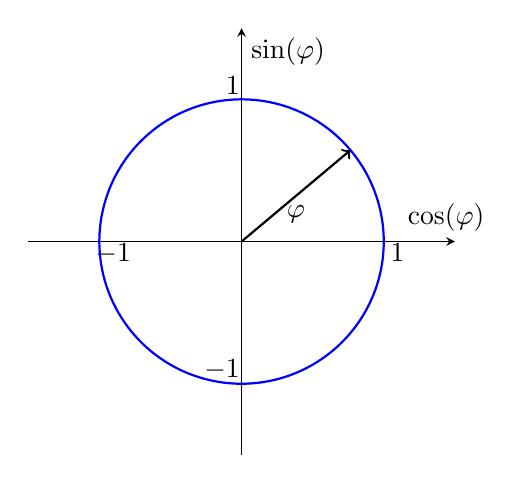
\begin{tikzpicture}
            \begin{axis}[
                axis lines=middle, 
                xlabel={$\cos(\varphi)$},
                ylabel={$\sin(\varphi)$},
                xlabel style={xshift=0.5cm},
                width=7cm, height=7cm,
                major grid style={line width=.2pt,draw=gray!50},
                minor grid style={line width=.1pt,draw=gray!20},
                xmin=-1.5, xmax=1.5,
                ymin=-1.5, ymax=1.5,
                xtick={-1, 0, 1},            % Manuelle Ticks auf der x-Achse
                ytick={-1, 0, 1},            % Manuelle Ticks auf der y-Achse
                tick label style={xshift=5pt, yshift=5pt}, % Verschiebt die Beschriftungen nach außen
            ]
            
            % Vektor einzeichnen
            \draw[thick, ->] (0,0) -- ({cos(40)}, {sin(40)}) node[above right] {};
            \node at ({0.5*cos(40)}, {0.5*sin(40)}) [below] {$\varphi$};
        
            % Kreis zeichnen
            \addplot[
                domain=0:360, 
                samples=200,  
                thick,
                color=blue,
            ]
            ({cos(x)}, {sin(x)}); 
            \end{axis}
        \end{tikzpicture}
    \end{minipage}
    \hspace{0.5cm}
    \begin{minipage}[t]{0.45\textwidth}
        \centering
        \begin{tikzpicture}
            \draw[->] (-2,0) -- (2,0) node[right] {}; 
            \draw[->] (0,-2) -- (0,2) node[above] {}; 
            \node at (-1.5,1.5) {$\cos\left(k \frac{\pi}{2}\right)$};
            \node at (-2,0) [left] {$2,6,\ldots$}; 
            \node at (2,0) [right] {$0,4,\ldots$}; 
            \node at (0,2) [above] {$1,5,9,13,\ldots$}; 
            \node at (0,-2) [below] {$3,7,11,15,\ldots$}; 

            % Kreuz bei jedem markierten Punkt
            \foreach \x/\y in {-1.5/0, 1.5/0, 0/1.5, 0/-1.5} {
                \draw[thick]
                    (\x,\y) +(-0.1,0.1) -- +(0.1,-0.1) % Diagonale des Kreuzes
                             +(-0.1,-0.1) -- +(0.1,0.1); % Andere Diagonale des Kreuzes
            }
        \end{tikzpicture}
    \end{minipage}
        
    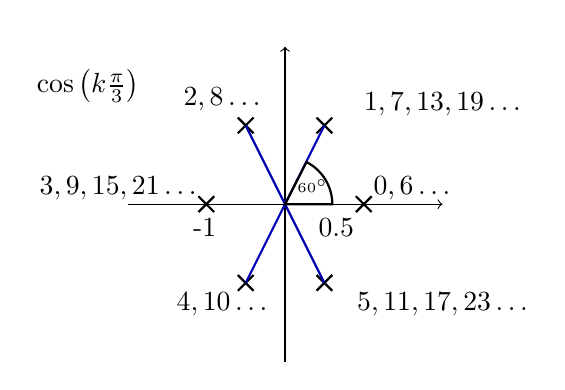
\begin{tikzpicture}
        \draw[->] (-2,0) -- (2,0) node[right] {}; 
        \draw[->] (0,-2) -- (0,2) node[above] {}; 
        \node at (-2.5,1.5) {$\cos\left(k \frac{\pi}{3}\right)$};
        \node at (-1,0.2) [left] {$3,9,15,21\ldots$}; 
        \node at (1,0.2) [right] {$0,6\ldots$}; 
        \node at (2,1) [above] {$1,7,13,19\ldots$}; 
        \node at (-0.8,1.6) [below] {$2,8\ldots$};
        \node at (-0.8,-1) [below] {$4,10\ldots$}; 
        \node at (2,-1) [below] {$5,11,17,23\ldots$};
        \node at (-0.75,-0.3) [left] {-1};
        \node at (1,-0.3) [left] {0.5};
        % Kreuz bei jedem markierten Punkt
        \foreach \x/\y in {-1/0, 1/0, 0.5/1, -0.5/-1, 0.5/-1, -0.5/1} {
            \draw[thick]
                (\x,\y) +(-0.1,0.1) -- +(0.1,-0.1) % Diagonale des Kreuzes
                         +(-0.1,-0.1) -- +(0.1,0.1); % Andere Diagonale des Kreuzes
        }
        \draw[thick, color=blue!70!black]
        (-0.5,1) -- (0.5,-1) -- cycle;
        \draw[thick, color=blue!70!black]
        (0.5,1) -- (-0.5,-1) -- cycle;
        \node[shift={(0.1,0)}, anchor=west] at ({0.5*cos(60)}, {0.5*sin(60)}) [below] {\tiny $60^\circ$};
        \def\drawArc#1#2#3{
        \draw[thick] (#1:0) -- (#1:#3) arc (#1:#2:#3) -- cycle;
    }
        % Beispiel: Kreissegment von 0 bis 60 Grad mit Radius 0.6
    \drawArc{0}{63}{0.6}{thick, color=blue!70!black};

    \end{tikzpicture}
    \hspace{2.3cm} % Abstand zwischen den beiden Diagrammen
    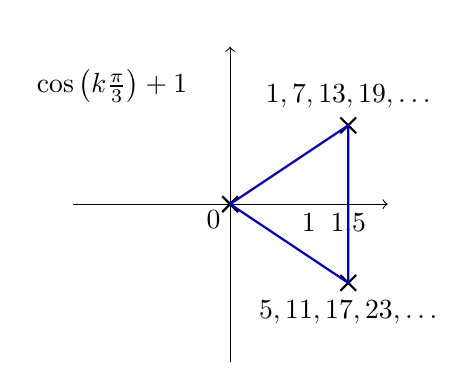
\begin{tikzpicture}
        % Koordinatensystem zeichnen
        \draw[->] (-2,0) -- (2,0) node[right] {}; 
        \draw[->] (0,-2) -- (0,2) node[above] {}; 
        \node at (-1.5,1.5) {$\cos\left(k \frac{\pi}{3}\right)+1$};
    
        % Beschriftungen an der x-Achse
        \node at (-0.00009,-0.2) [left] {0};
        \foreach \x in { 1, 1.5} {
            \node at (\x, 0) [below] {\x};
        }
    
        % Beschriftungen an spezifischen Punkten
        \node at (1.5,1.1) [above] {$1,7,13,19,\ldots$}; 
        \node at (1.5,-1.1) [below] {$5,11,17,23,\ldots$}; 
    
        % Kreuz bei jedem markierten Punkt
        \foreach \x/\y in {0/0, 1.5/1, 1.5/-1} {
            \draw[thick]
                (\x,\y) +(-0.1,0.1) -- +(0.1,-0.1) % Diagonale des Kreuzes
                         +(-0.1,-0.1) -- +(0.1,0.1); % Andere Diagonale des Kreuzes
        }
    
        % Verbindungslinien zwischen den Punkten
        \draw[thick, color=blue!70!black]
            (0,0) -- (1.5,1) -- (1.5,-1) -- cycle;
    \end{tikzpicture}
    \caption{Graphical solution of the cos terms.}
    \label{fig:Graphical solution of the cos terms}
\end{solutionfigure}
 
\end{solutionblock}


\subtask{Based on \autoref{sub:DecomposeVoltage}, calculate the fundamental amplitude $\hat{i}_\mathrm{a}^1$ using a vector diagram and complex alternating current calculations. 
From this, determine the total active power converted in the load.}
\begin{solutionblock}
\end{solutionblock}